
\section{Psychometrics}
In the animated 1937 classic \textit{Clock Cleaners}, Mickey Mouse, Donald Duck, and Goofy are working as janitors in a clock tower. As usual, Goofy is dimwitted and carefree, Donald Duck gets fits of anger, and Mickey Mouse is kind and compassionate. Goofy mistakes a statue for a lady, Donald Duck throws a temper tantrum at a spring, and Mickey Mouse does everything he can to save Goofy from falling to certain death. This is not the only animated movie were these characters behave like this. Donald Duck's fiery temper -- and bad luck -- is what he is known for, and something you would expect to see in any movie featuring him. Likewise, Goofy is always thickheaded. We say that these characters have \textit{stable psychological traits}. And real humans have them too. There are people you would describe as temperamental. In almost every situation, they are more prone to getting angry than others.

Psychometrics is about the study and quantification of psychological traits such as temperament. These traits cannot be directly measured though. Even if you think every individual has, in Platonic sense, a real variable $Z$ called "temperament", you would not be able to measure it directly. For these traits are not observable, they are \textit{latent}. Instead of observing $Z$ directly, we observe a random vector $X$ of proxies for $Z$. In most cases these proxies are responses to a questionnaire, usually on \emph{Likert items}. A Likert item is the response to a question with ordered alternatives ranging from e.g. strongly disagree to strongly agree. Table \ref{tab:IPIP} shows five questions from the International Personality Item Pool \parencite{Goldberg1992-hp}, all of them supposedly related to the trait \textit{agreeableness}.

\begin{table}
\caption{\label{tab:IPIP}Five questions loading on \textit{agreeableness} from the International Personality Item Pool}
\noindent \begin{centering}
\begin{tabular}{lccccc}
 & $1$ & $2$ & $3$ & $4$ & $5$\tabularnewline
I Am indifferent to the feelings of others.  & $\bigcirc$ & $\bigcirc$ & $\bigcirc$ & $\bigcirc$ & $\bigcirc$\tabularnewline
I inquire about others' well-being. & $\bigcirc$ & $\bigcirc$ & $\bigcirc$ & $\bigcirc$ & $\bigcirc$\tabularnewline
I know how to comfort others. & $\bigcirc$ & $\bigcirc$ & $\bigcirc$ & $\bigcirc$ & $\bigcirc$\tabularnewline
I love children. & $\bigcirc$ & $\bigcirc$ & $\bigcirc$ & $\bigcirc$ & $\bigcirc$\tabularnewline
I make people feel at ease.  & $\bigcirc$ & $\bigcirc$ & $\bigcirc$ & $\bigcirc$ & $\bigcirc$\tabularnewline
\end{tabular}
\par\end{centering}
\vskip7.0pt
\noindent \centering{}{\scriptsize{}1, Very Inaccurate; 2, Moderately
Inaccurate; 3, Neither Accurate Nor Inaccurate; 4, Moderately Accurate;
5, Very Accurate}{\scriptsize\par}
\end{table}

These questions are said to \textit{load on} the personality trait agreeableness. A person strongly agreeing with ``Am indifferent to the feelings of others.'' is likely to be disagreeable, and his affirmative answer is likely to be caused by his disagreeableness. Psychometrics is about using questions such as these to infer, numerically, how agreeable someone is. The questions serves as proxies for the latent variable, and it is the latent variable we are actually interested in. The answers to the individual questions are not too interesting in and of themselves.

To be able to connect proxies to their latent variables, will need a statistical model. The most popular model is the linear model. Here $Y$ is a $J$-ary vector and
\begin{equation}
Y=\lambda Z+\Psi^{1/2}\epsilon,\label{eq:one-factor model}
\end{equation}
where $\Lambda$ is a real matrix of \emph{factor loadings}, $\Psi$ is a positive definite matrix, $\epsilon$ is a $J$-ary vector of uncorrelated error terms, and both $Z$ and $\epsilon$ have finite variances. This is the linear factor model. Of particular interest is the \textit{one-factor model}, where $Z$ is scalar and $\Lambda = \lambda$ a vector of loadings.

The linear factor model is a member of the wider class of generalized item response models \parencite{Mellenbergh1994-iy}, which encompasses most psychometric models \parencite[Chapter 3.1]{Borsboom2005-iq}. A generalized item response model is similar to a generalized linear model. Let $X$ be a vector of covariates, $Z$ be a vector of latent variables, $g$ a monotone link function, and $Y$ the $J$-ary vector of responses. Then 
\begin{equation}
g(E[Y_{j}])=\lambda_{j}^{T}Z+\beta_{j}^{T}X,\quad(j=1,\ldots J)\label{eq:GLIRT model}
\end{equation}
is a generalized item response model.

The most important feature of psychometric models is the reversed roles of regressors and covariates. In a usual regression model, the left hand side is unknown and the input to the right hand side is known. For instance, when we regress gross domestic product on some other economic indicators, we wish to predict gross domestic product from those other indicators. We can imagine a situation where we know the economic indicators and make a guess about gross domestic product. 

In psychometrics this situation is turned on its head. We know the regressors but not all of the covariates. In the words of \textcite[p. 61]{Borsboom2005-iq}, models in psychometrics are \emph{reflective}, not \emph{formative}. In a formative model, a variable $Y$ is defined in terms of its indicator. For instance, socio-economic status is defined in terms of variables such as income, education level, and neighborhood quality. But socio-economic status does not cause them, it is merely a summary \parencite[p. 62]{Borsboom2005-iq}. On the other hand, agreeableness causes the responses to the questions in Table \ref{tab:IPIP}. Figure \ref{fig:dag} shows formative and reflexive models using directed graphs, where directed arrows are interpreted causally.

\begin{figure}
\noindent \begin{centering}
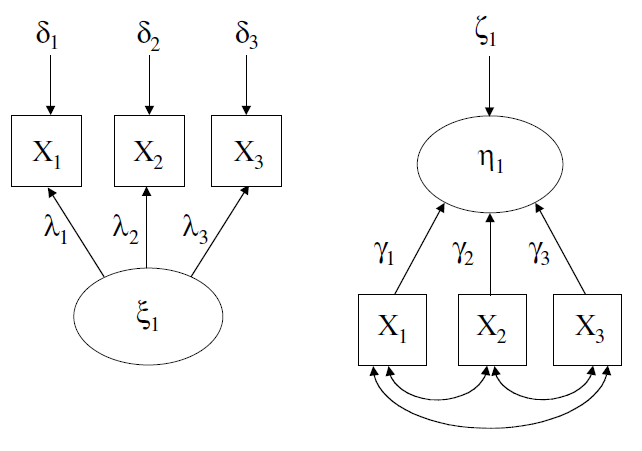
\includegraphics[scale=0.5]{chunks/borsboom}
\par\end{centering}

\caption{\label{fig:dag}(left) A reflexive model where the latent variable $\xi_{1}$ causes the observed $X_{i}$s. (right) A formative model where $\eta_{1}$ is defined in terms of the $X_{i}$s. This figure is taken from \textcite[p. 61]{Borsboom2005-iq}.}
\end{figure}

When we have a psychometric model such as the one-factor model, we want to estimate the latent $Z$. Disregarding potential covariates $X$, an estimator of $Z$ must be based on the vector of observed variables $Y$ only. That is, $\hat{Z}=\phi(Y)$, a function of the observed variables $Y$. For generalized item response models, the maximum likelihood estimator of $Z$ or its posterior mean are common estimators of $Z$. These quantities are only defined when we make parametric assumptions about all random variables involved. But the linear one-factor model is a semi-parametric model, and the maximum likelihood estimator of $Z$ need not exists. The most widely used estimator of $Z$ in psychology is the \emph{sum
score}, $\hat{Z}=\sum_{i=1}^{k}Y_{i}$, and the mean squared error-optimal linear combination $\hat{Z}=\sum_{i=1}^{k}v_{i}Y_{i}$ is popular too. Both of these make sense mainly in the linear one-factor model. 

The three fundamental questions of psychometrics are:
\begin{enumerate}
\item \textbf{Model fit}. Is the model a good approximation to reality? Are the structural and parametric assumptions defensible? Model fit in structural equation modelling is usually evaluation through model fit indices, for instance $\chi^{2}$-tests. \parencite[Chapter 15]{Mulaik2009-gc}.
\item \textbf{Reliability}. Is $\hat{Z}$ a good estimator of $Z$, assuming the model is correct? If so, the estimator is reliable. In the linear one-factor model, the reliability is most often measured by calculating coefficient alpha \parencite{Cronbach1951-in}, a statistic related to the squared correlation $\Cor^{2}(Z,\hat{Z})$ between $Z$ and $\hat{Z}$ when $\hat{Z}$ is a sum-score.
\item \textbf{Validity}. Is $Z$ what we want it to be? Even if the model is correct, $Z$ might be something else than what we would like it to be. For instance, the five questions of Table \ref{tab:IPIP} should be related to the personality trait agreeableness. But is true? Maybe they measure some other psychological trait, such as irritability, intelligence, or even a physical trait such as height. Assuming personality traits such agreeableness exists, which not every psychometrician agrees with, there are some methods to check this. The techniques are often extrastatistical, and the application of them is called \emph{validation}. \parencite[Chapter 6]{Borsboom2005-iq}
\end{enumerate}

\subsection{Reliability}

There is a mismatch between the mathematical definition of reliability and what psychologists think reliability is. The common definition of reliability is slightly different from correlation definition above. In our terminology, \textcite[Equation 3]{Raykov2019-yr} defines the reliability of $\hat{Z}$ as a measurement of $Z$ as
\begin{equation}
\rho=\frac{\Var Z}{\Var\hat{Z}}\label{eq:rakov-reliabiliy}
\end{equation} Under the linear model \eqref{eq:one-factor model}, $\rho = \Cor^2(Z,\hat{Z})$ when $Z$ is a linear predictor of $Z$ with zero mean, which happens when $Z$ is the sum-score $\hat{Z}=\sum_{i=1}^{k}Y_{i}$ or the mean squared error-optimal linear combination $\hat{Z}=\sum_{i=1}^{k}v_{i}Y_{i}$.

Both the correlation definition and ratio of variance definition of reliability are straight-forward. Both are defined relative to statistical model, and both inform us about the quality of $\hat{Z}$ as a predictor of $Z$. But it is common for psychologists to hope for much more. For instance, \textcite{McNeish2018-vu} wrote that
\begin{quote} 
[...] researchers often report a measure of reliability to demonstrate that the items composing the measure are reliable, meaning that the scores based on the items are reasonably consistent, the responses to the scale are reproducible, and that responses are not simply comprised of random noise. Put another way, a reliability analysis provides evidence that the scale is consistently measuring the same thing [...]
\end{quote}

It is hard to reconcile all these claims with the definition of reliability, except that the responses cannot be random noise only. The claim that reliability analyses provide evidence that the scale consistently measure the same thing makes some researchers call reliability coefficients measures of internal consistency. This notion is incorrect, as the reliability coefficient cannot be used to differentiate between factors model with one or more factors \parencite[]{McDonald1981-xz}.

I do not claim that reliability coefficients are useless. If you have reason to believe in your model, a high reliability coefficient is nice to have, as it allows you to predict $Z$ well. But just as $R^2$, it is not a measure of model fit \parencite{Helland1987-eb}. Just as the $R^2$ can be small even if the linear model fits exactly, the reliability coefficient can be small even when the responses to the scale are reproducible and the scale measures the same thing. 

Reliability coefficients are ubiquitous in psychology. The most used coefficient is coefficient alpha, also known as Cronbach's alpha. This coefficient is the reliability for the sum-score under the linear one-factor model \eqref{eq:one-factor model} assuming $\tau$-equivalence, i.e., $\lambda_i = \lambda_j$ for all $i,j$. Its definition is 
\begin{equation}
\hat{\alpha}=\frac{k}{k-1}\left(1-\frac{\tr{S}}{\boldsymbol{1}^{T}S\boldsymbol{1}}\right),\label{eq:sample coefficient alpha}
\end{equation}
where $k$ is the size of $Y$, the vector $\boldsymbol{1}$ is a $k$-ary vector of only ones, and $S$ is the covariance matrix of $Y$. It is straight-forward algebra to verify that coefficient alpha equals the reliability for the sum-score $\hat{Z}$ under the $\tau$-equivalent model.

Cronbach's \citeyear{Cronbach1951-in} paper on coefficient alpha has $45673$ Google scholar cites as of August 2020. It is the third-most cited paper in psychology and in the top-hundred of the most cited papers in any field \parencite{McNeish2018-vu}. Whenever a reliability coefficient is reported, there is a $75\%$ chance it's coefficient alpha.

Reliability coefficients are routinely reported in investigations of psychometric scales. For example, \textcite{Marx1978-rf} administered \enquote{three self-report measures of self-concept} to \enquote{488 sixth grade children as the basis for a [...] self-concept measurement.} They found that the first self-report measure had sample coefficient alpha $0.56$, the second $0.55$, and the third $0.67$. 

Reliability coefficients are frequently debated by psychologists and psychometricians. A decent introduction to the literature is McNeish's \citeyear{McNeish2018-vu} attack on coefficient alpha together with the comments of \textcite{Raykov2019-yr} and \textcite{Savalei2019-se}. Psychometrika Volume 74, Issue 1 of 2009 is a relatively recent issue devoted mainly to coefficient alpha. A potential difficulty for statisticians trying to enter this fields are the two cultures of psychometrics, discussed by e.g. \textcite{Borsboom2005-iq}. One one hand are researchers working in the framework of latent variables, which is accessible to statisticians, as they work with explicit statistical models. But the majority of psychologists have been trained in the classical test theory of \textcite{Lord1968-ax}, which is slightly more esoteric to a statistician. Luckily, classical test theory can be subsumed under latent variable theory without much work.

\subsection{Normal-ogive models}
\label{subsec:Normal-ogive models}

A probit regression can written down as
\begin{eqnarray*}
Z\mid X & \sim & \beta^{T}X+\epsilon\\
Y\mid Z & \sim & 1[Z>0]
\end{eqnarray*}
provided only that $\epsilon$ is standard normal. Here we have a latent continuous variable $Z$, never observed, that captures the true regression relationship with $X$. Sadly, we only observe $Y$, with the associated loss of power. Probit regression is not alone in having this interpretation, as the famous logit model has the same interpretation, but with a logistically distributed $\epsilon$ in place of the normally distributed $\epsilon$. These models are popular, likely because the make more sense for binary data than the obvious competitor, linear regression.

Most psychometric data is on a Likert scale, usually on the range $1$ -- $5$ or $1$ -- $7$. These data are ordinal, and we are usually not justified in interpreting them as real numbers with the ordinary distance metric. But the popular linear factor model is best understood as modelling real numbers. How can we reconcile the linear factor model with Likert scale items?

The most common answer is to pretend the Likert scale items are real numbers, and use the linear factor model directly. Another popular answer is to use thresholding as in the probit and logit model.  

Recall the linear factor model
\begin{equation}
X=\Lambda Z+\Psi^{1/2}\epsilon,      \tag{\ref{eq:one-factor model}}
\end{equation}
where $\Lambda$ is a matrix, $\Psi$ positive definite, and $\epsilon$ uncorrelated with $Z$. Consider the scenario when we do not observe the $X$s directly, but rather $X$s discretized into $m$ categories according to
\begin{equation}
Y=j1[\tau_{(j-1)}\leq X\leq\tau_{j}],\quad j = 1, \ldots,m. \label{eq:discretization model}
\end{equation}
Here $-\infty=\tau_{0}<\tau_{1}<\ldots<\tau_{m}=\infty$
are thresholds.

If $X$ is multivariate normal, model (\ref{eq:discretization model})
is a \textit{normal-ogive model} \parencite{Swaminathan2016-rg}, also known as a discretized factor analysis model \parencite{Takane1987-pq}. Estimating of normal-ogive models is not much more involved than estimation of linear factor models. The correlation matrix of $X$ is called the \textit{polychoric correlation matrix}, it is identified and relatively straight-forward to estimate \parencite{Olsson1979-ti}. Using this estimated correlation matrix, the parameters $\Lambda$ and $\Psi^{1/2}$ can be calculating using e.g. minimum square procedures. The polychoric correlation matrix can also be used as input to coefficient alpha \eqref{eq:sample coefficient alpha} instead of the sample covariance matrix, yielding the \textit{ordinal alpha} \parencite{Zumbo2007-ap}. 

Be aware that it is impossible to verify the distributional assumptions about $X$, as we do not observe it, only $Y$. While some distributions of $X$ are incompatible with normality, there are a plethora of distributions compatible with $X$ that are not normal even when $X$ is compatible with normality \parencite{Foldnes2020-ma}. In this regard, testing $X$ for normality is impossible in the same sense as non-parametric testing of the mean from Theorem \ref{thm:bahadur-savage}.